\subsection{Implementation}
\label{sec:impl}

We implemented the outlined solution concept in a Python script. This script automatically fetches, processes and analyses the log files and creates a classification model that is based on the extracted information. The following tools are used for implementation:

\begin{description}

\item[\textbf{Technology.}] Python is a general-purpose, high-level programming language. It is open source, easy to use and offers various third party modules\footnote{https://www.python.org/}.

\item[\textbf{Machine Learning.}] The Scikit Learn module is used for machine learning\footnote{http://scikit-learn.org/stable/}. We used \glspl*{dt} for classification and regression. \Glspl*{dt} are a supervised learning method whose goal is to create a model that predicts a target feature of variable by inferring existing rules from the data.

\item[\textbf{Natural Language Processing.}] The Natural Language Toolkit (NTLK) offers methods to extract additional information from everyday communication. Among others, we rely on the \emph{bag of words} technique that analyzes word occurrences\footnote{http://www.nltk.org/book/ch00.html}.

\end{description}

Next, we discuss the data selection criteria. While there are many accessible code repositories, picking a dataset of appropriate size and quality proves to be rather challenging. We need to consider:

\begin{description}

\item[\textbf{Diversity}.] Classification on a single repository might not produce a generally applicable result, whereas using more repositories increases complexity.

\item[\textbf{Size}.] Individual repositories' size is determined by the number of commits.

\item[\textbf{Roles}.] The real roles of the contributors of a repository is required for certain classification steps and the verification of results.

\item[\textbf{Type}.] Differences in organizational aspects of the projects: the type of the development team (e.g. professional or hobby), type of software (e.g. proprietary or open-source), and type of platform (e.g. private server or public repository hosting service) can influence the way repositories are used.

\item[\textbf{Backend}.] There exists a plethora of version control systems, each with their unique characteristics and formats. The approach should be able to handle popular systems including Subversion (SVN), Git, and Mercurial.

\end{description}

Based on these criteria, we selected three repositories for analysis, each with thousands of commits:

\begin{enumerate}

\item Main code repository of the company Infinica. Proprietary software. VCS: Mercurial

\item ProM Sourceforge project repository. Open source software. VCS: SVN

\item Camunda GitHub project repository. Open source software. VCS: Git

\end{enumerate}


These repositories cover a broad range of the above mentioned differences. The necessary role information was reviewed by interviews with the main contributors of these projects. While two repositories were openly available, the third was granted a direct access from within the company.

%First of all, browsing through the commit messages created an understanding of the structure of the log files, the type of information available for extraction and the way VCS commits are typically used in the different projects. They contain the most useful information but are also the least predictable factor, because there are no general rules on how to formulate such a message. 

An initial screening of commit messages in the repositories revealed that there is useful information within most of the messages, but the variance regarding the style and content of the messages is high between commits and users.
From the messages, certain words and phrases can be extracted, which can be linked to a specific class. In a next step, the log files were preprocessed removing commits and/or users with faulty information, merging users with several accounts and anonymizing the data if required. 

%The first step of creating the algorithm, once the log files were obtained and their basic structure was known, is to transform them into a common in-memory object model. 
To unify the different systems, we create a shared object model to store the relevant information.
%Three different functions, providing the same output for different input formats, were required to cover all three systems (Git, Svn, Mercurial). 
This model consists of a commit object for each commit in the log, consisting of an id, an author, a message, a timestamp and lists of all added, modified and deleted files. From this model it is possible to derive a second model consisting of the users, by aggregating the information for each author name occurring in the commits.

In the following, we present two ways to tackle the problem of classification of users into their respective roles. First, the \emph{user-based} approach focuses on the users at an aggregated level. Second, the \emph{commit-based} approach classifies individual commits to allow for a finer grained classification. 

%For further analysis and classification steps, efforts have been split up into two approaches. The first one focuses purely on the users and the features deductible for them. We soon realized though that this method, while providing some promising insights, had certain limitations and left out some potentially valuable information. Therefore a second approach was incorporated taking a closer look at the individual commits. The two approaches are outlined in more detail in the following sections.

\subsection{User-based Approach}

The main idea of this approach is to use clustering in order to find potential user classes and build a classification model based on those clusters, which represent a comprehensible, existing class of users. As a clustering method we used k-means.

The first step is feature selection. We identified the following features per user.

\begin{itemize}

\item Total number of commits.

\item Timeframe: the time between the first and last commit of the user (approximates the time a user has been working on a project).

\item Commit frequency: total number of commits divided by the time frame. Represents the number of commits a user makes within a certain period of time (e.g. day, month).

\item Commit message length: average length of commit messages in number of words.

\item Keyword occurrence: how often a certain word (e.g. "test", "fix") is used relative to the total number of words.

\item Number of added/modified/deleted files.

\item Affected file types: how often a file with a certain format (e.g. .java, .html) are modified by a user, relative to the total number of modified files.

\end{itemize}


%In order to find useful clusters, an experimentation with different combinations of features is necessary. For each of these combinations the optimal cluster number has to be found. While the clustering and optimizing tasks can be automated, the clusters have to be evaluated manually. This makes it impossible to test all possible combinations of features, especially when including the keyword occurrence numbers, as the list of keywords with potential value was far too large. Combinations that promise useful results are selected. Evaluation is done using plots as well as looking at the raw data to find connections between the identified clusters and the existing classes in the sample data.


From the clusters generated with this method, classification models are built using the decision tree method. This method uses tree graphs for representing the model. Each branching in the tree represents one decision based on the characteristics of a certain data point. Each leaf of the tree stands for a class. The classification is done by going through the tree for each data point and assigning it the class of the leaf it reaches. The models are trained for the three data sets individually. For verification of their quality, the models are cross validated with the other data sets respectively.


\subsection{Commit-based Approach}

There are multiple reasons for exploring a second approach in addition to the user clustering. As already mentioned above, the research led to the conclusion that in many cases a user can have multiple roles or execute many tasks not belonging to her primary role. This kind of use case is hard to cover using only the simple clustering method. Another reason is that a lot of information is lost when aggregating the commit information for users. This leads to the idea of classifying individual commits.


The algorithm iterates over commits and tries to assign types to them. The types are assigned based on the analysis of the commit message, and on the file extensions. The commit message is searched for certain keywords and phrases which are connected to types. The file extensions are searched for known file types fitting to a commit type. There are certain overlaps between commit types, for example the type addition can be a development or test commit. In those cases where one identified type is a more specific description for another, only the more specific one is included into the further analysis. The identified commits and the related keywords and file types are listed in \Cref{tab:keywords}.

\begin{table}[]
   \centering
   \caption{Keyword lemmas used for classification}
   \label{tab:keywords}
   \begin{tabular}{@{}m{.2\columnwidth}m{.7\columnwidth}@{}}
      \toprule
      \textbf{Class} & \textbf{Keywords}                                                                                               \\ \midrule
      Test           & test testcase test case unittest unit test integrationtest fitnesstest fitness test                                     \\
      Development    & implement improve update script                                                                                 \\
      Web            & web spring http http rest html css servlet                                                                      \\
      Backend        & engine                                                                                                          \\
      Maintenance    & bugfix fix patch cleanup clean up clean                                                                         \\
      Refactor       & refactor rename move revert                                                                                     \\
      Documentation  & document javadoc readme userguide guide tutorial faq translate doc i18n *.txt *.doc *.docx *.text *.tex *.pdf \\
      Design         & style icon font layout *.png *.svg *.jpg                                                                        \\
      Build          & build compile release                                                                                           \\
      Data           & data database sql postgre postgresql                                                                            \\
      Tool           & tool library framework depend upgrade                                                                           \\
      Addition       & add new create                                                                                                  \\
      Removal        & delete remove                                                                                                   \\
      vcsManagement  & svn git mercurial                                                                                               \\
      Automated      & automated release, automated nightly                                                                            \\
      Merge          & merge                                                                                                           \\ \bottomrule
   \end{tabular}
\end{table}

After assigning the commit types, the commits can be aggregated for the individual users resulting in the absolute occurrence numbers of each type for each user. Dividing each of these values by the total number of commits of the user, we get percentages for each type. These percentages tell how the work of a user is distributed among the different kinds of tasks which appear in a VCS. These user profiles are a form of classification, which is not as simple and concise as assigning one definite class for each user, but has the advantage of covering secondary roles and minor tasks. They can be useful for analyzing smaller project teams with multiple roles for one user.

The classification task is done on user profiles. A table of user profiles is created and a role for each user manually inserted, based on the role information of the data sets. For this part the Infinica data set is used, because it is the one with the most extensive information base and it has the most diverse and comprehensive set of roles among the shosen repositories. Four roles are assigned to the Infinica users: Web developers, other developers, testers and support. The last one is an aggregation of users who have different official roles but contribute in the VCS mainly in form of minor, supportive tasks.

The classification task was done in two ways: 1. Manual analysis of the table and derivation of rules by looking for similarities between users with the same role. 2. Automated classification in line with our original concept. For the latter the decision tree method is used. In this case the commit type percentages are used as features and the manually assigned roles as classes. The resulting decision tree model was validated against the ProM and Camunda data sets.


The final algorithm including retrieval, processing and analysis of data as well as classification and verification, consists of roughly 700 lines of code. The results for the two approaches are discussed below.


\section{Evaluation}

In the first step of the user-based approach, the most expressive features of the Infinica data set were identified. The solution was tested on the Infinica data set due to the immediate availability of detailed information about the log file. The best results were achieved with the combination of the commit frequency and the occurrence numbers of test related keywords.


The commit frequency is a strong indicator of developers. Moreover, it also differentiates between the working preferences of the developers. The group with the lower frequencies tends to work locally on their machines and pushes their work when it is finished. Whereas, the developer group frequently pushes incremental changes to the repository, so that everybody is updated and works with the latest code.


Test-related keywords can not only identify testers, but also differentiate between their expertise. The sum of the words "test", "tested", "testing", "tests" suffices to make a distinction between testers and developers. Additionally, manual testers use these words less often than their technical counterparts, who are more focused on automation.


The first part of the commit-based algorithm implementation, i.e., the commit classification, was successfully tested on all three data sets combined. For all three sets we achieved a similar coverage (percentage of commits which could be assigned some type). For Infinica the coverage was 88,94\%, for Camunda it was 90,25\% and for ProM 86,65\%.

While the user profiles were originally intended as an intermediary step and a means to verify and improve the quality of our approach, they proved to be a useful perspective on user roles, beyond the simple categorisation using a single class. Especially when using a graphical representation such as the pie charts which can be seen in \Cref{fig:developer} and \Cref{fig:tester}, the commit distribution provides an interesting insight in the actual roles and tasks of users.

\begin{figure*}[ht]
   \centering
   \begin{subfigure}[t]{.5\textwidth}
      \centering
      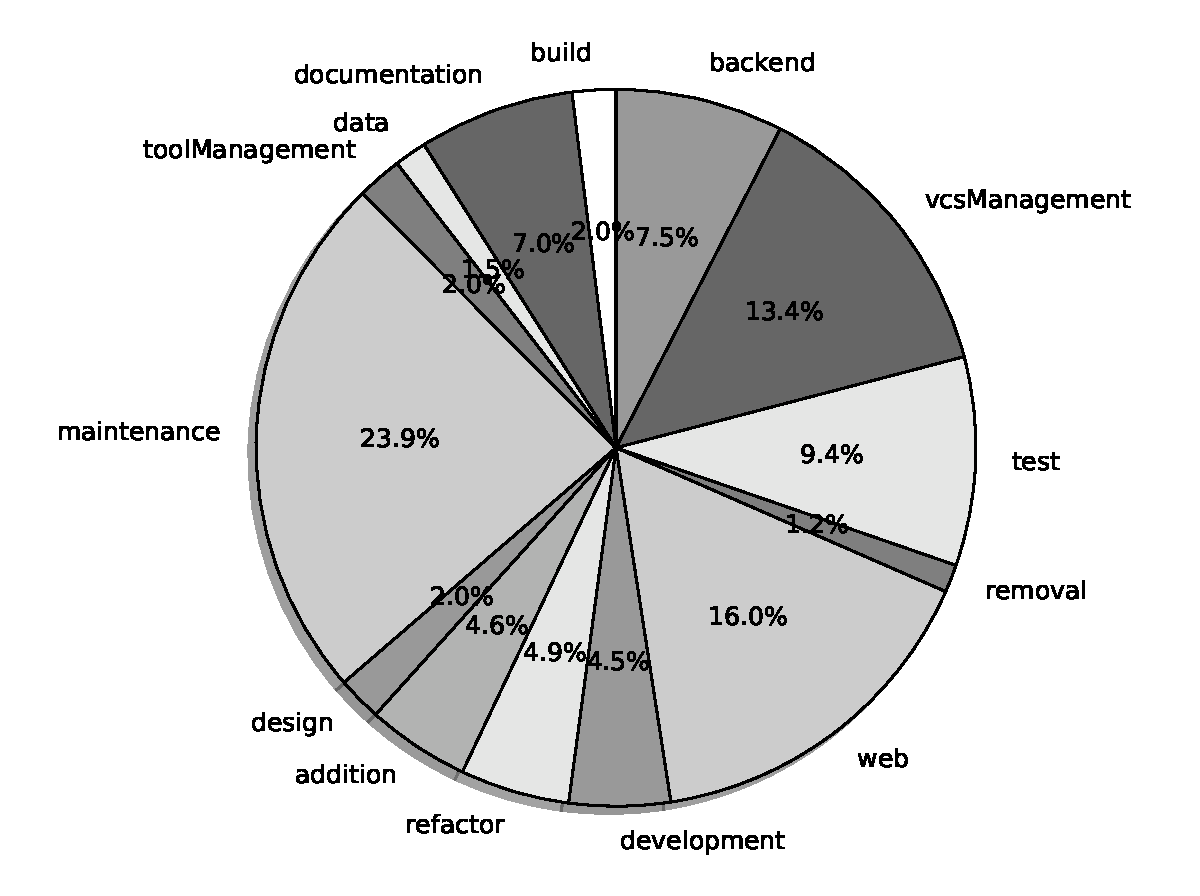
\includegraphics[width=\linewidth]{ResourceClassification/figures/infinica_developer.pdf}
      \caption{User profile for a backend developer}
      \label{fig:developer} 
   \end{subfigure}%
   \begin{subfigure}[t]{.5\textwidth}
      \centering
      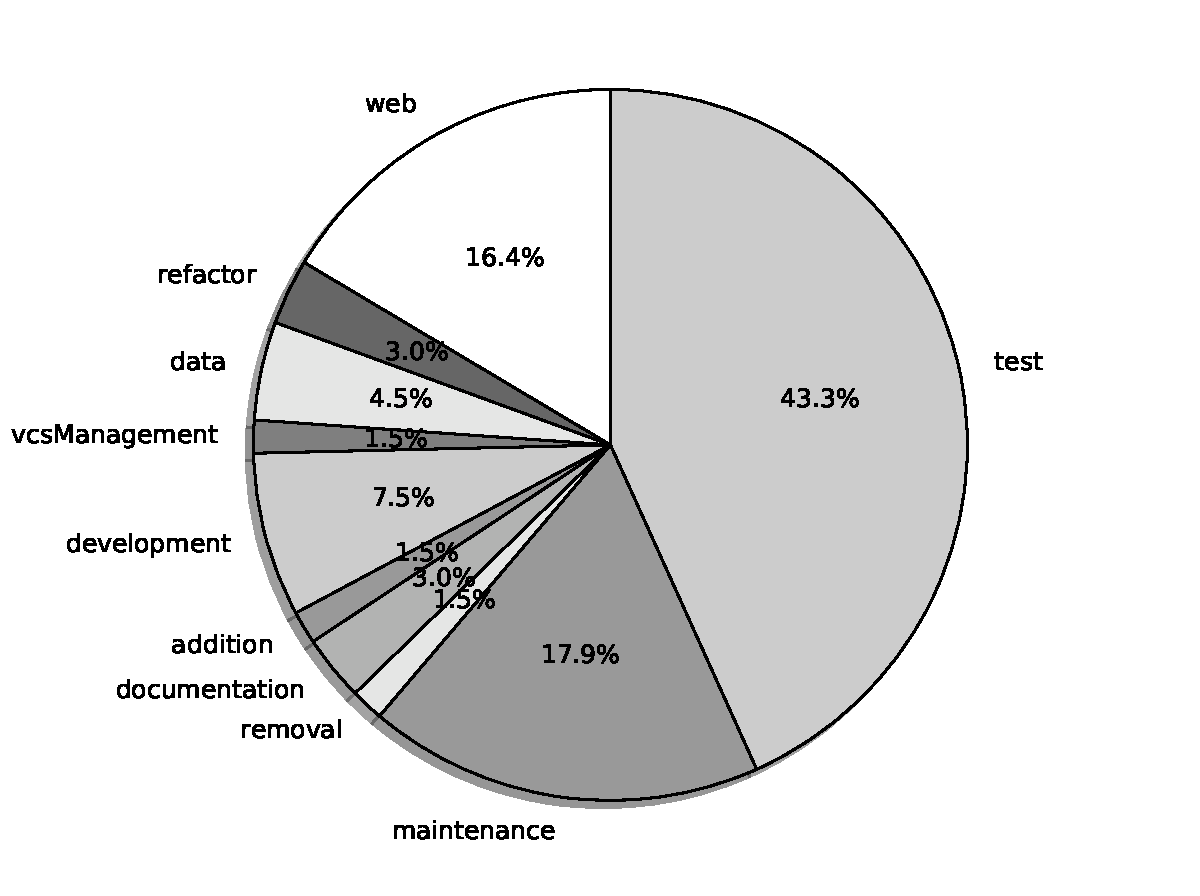
\includegraphics[width=\linewidth]{ResourceClassification/figures/infinica_tester.pdf}
      \caption{User profile for a tester}
      \label{fig:tester} 
   \end{subfigure}
   \caption{Commit distributions of the Infinica dataset}
   \label{fig:test}
\end{figure*}

\begin{figure}[h]
	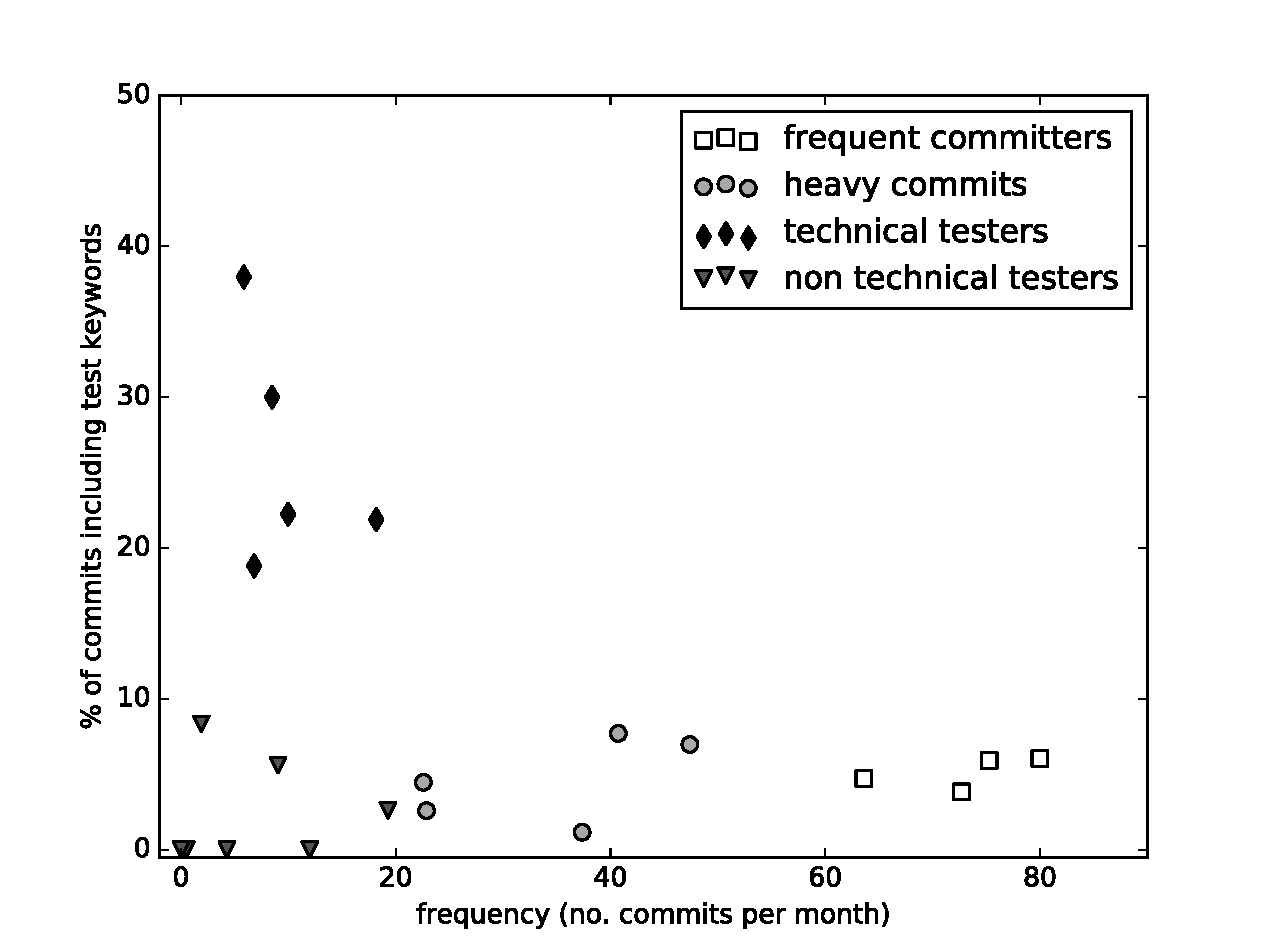
\includegraphics[width=\columnwidth]{ResourceClassification/figures/infinica4k_black.pdf}
	\caption{Scatterplot with highlighted clusters (k=4) based on the Infinica data set.}
	\label{fig:infinica4k}
\end{figure}

The Infinica dataset is divided successfully into expressive classes with k-means clustering with a k=4 shown in \Cref{fig:infinica4k}. The developers (light grey circle and white square) are split off based on their higher frequency in the first step of the decision tree and the following classes are derived:

\begin{itemize}

\item \textbf{Developers - frequent committers:} The square cluster is comprised  of developers which push every change to the repository.

\item \textbf{Developers - heavy commits:} The circle cluster contains developers who work on their local machine and push less frequently. However, they have bigger commits containing more changes.

\item \textbf{Testers - technical:} Testers focused on automating the testing process are in the diamond cluster. They are solely senior developers but not all of them are situated in this group.

\item \textbf{Testers - non technical:} The triangle cluster is comprised of less technical testers which tend to do more manual testing. Additionally, it includes the professional services team.

\end{itemize}

\Cref{tab:user-profiles2} shows an excerpt of the user profiles and role assignments for the Infinica data set. The commit types development, backend, maintenance and refactor have been merged to a single type development, as the other, more specific types provided no additional value in this case. Also the types "addition", "removal" and "merge" have been omitted due to a lack of semantic meaning. The data visible in the table was used for the manual classification as well as the creation of the decision tree model.

% Please add the following required packages to your document preamble:
% \usepackage{booktabs}
\begin{table*}[]
   \centering
   \caption{Excerpt from user profiles with roles for Infinica data set}
   \label{tab:user-profiles2}
   \begin{tabular}{@{}rrrrrrrrrc@{}}
      \toprule
      \multicolumn{1}{c}{\textbf{\begin{tabular}[c]{@{}c@{}}test \\ \%\end{tabular}}} & \multicolumn{1}{c}{\textbf{\begin{tabular}[c]{@{}c@{}}development \\ \%\end{tabular}}} & \multicolumn{1}{c}{\textbf{\begin{tabular}[c]{@{}c@{}}web \\ \%\end{tabular}}} & \multicolumn{1}{c}{\textbf{\begin{tabular}[c]{@{}c@{}}documentation \\ \%\end{tabular}}} & \multicolumn{1}{c}{\textbf{\begin{tabular}[c]{@{}c@{}}vcsManagement \\ \%\end{tabular}}} & \multicolumn{1}{c}{\textbf{\begin{tabular}[c]{@{}c@{}}build\\ \%\end{tabular}}} & \multicolumn{1}{c}{\textbf{\begin{tabular}[c]{@{}c@{}}toolManagement\\ \%\end{tabular}}} & \multicolumn{1}{c}{\textbf{\begin{tabular}[c]{@{}c@{}}data\\ \%\end{tabular}}} & \multicolumn{1}{c}{\textbf{\begin{tabular}[c]{@{}c@{}}design\\ \%\end{tabular}}} & \textbf{\begin{tabular}[c]{@{}c@{}}class\\ name\end{tabular}} \\ \midrule
      6.07                                                                            & 39.49                                                                                  & 26.40                                                                          & 7.94                                                                                     & 0.23                                                                                     & 3.27                                                                            & 0.70                                                                                     & 0.23                                                                           & 11.21                                                                            & dev                                                           \\
      9.41                                                                            & 40.90                                                                                  & 15.99                                                                          & 7.00                                                                                     & 13.37                                                                                    & 1.96                                                                            & 2.04                                                                                     & 1.46                                                                           & 2.00                                                                             & dev                                                           \\
      3.83                                                                            & 26.78                                                                                  & 44.70                                                                          & 2.90                                                                                     & 4.70                                                                                     & 3.93                                                                            & 0.60                                                                                     & 2.95                                                                           & 6.01                                                                             & webdev                                                        \\
      0.00                                                                            & 28.07                                                                                  & 52.28                                                                          & 2.46                                                                                     & 0.00                                                                                     & 5.26                                                                            & 1.40                                                                                     & 0.35                                                                           & 8.42                                                                             & webdev                                                        \\
      43.28                                                                           & 28.36                                                                                  & 16.42                                                                          & 2.99                                                                                     & 1.49                                                                                     & 0.00                                                                            & 0.00                                                                                     & 4.48                                                                           & 0.00                                                                             & tester                                                        \\
      23.99                                                                           & 27.73                                                                                  & 15.26                                                                          & 7.79                                                                                     & 0.00                                                                                     & 2.49                                                                            & 1.56                                                                                     & 1.25                                                                           & 4.67                                                                             & tester                                                        \\
      0.00                                                                            & 7.94                                                                                   & 38.10                                                                          & 0.00                                                                                     & 38.10                                                                                    & 1.59                                                                            & 4.76                                                                                     & 0.00                                                                           & 9.52                                                                             & support                                                       \\
      1.19                                                                            & 3.39                                                                                   & 46.15                                                                          & 1.61                                                                                     & 46.15                                                                                    & 0.08                                                                            & 0.17                                                                                     & 1.19                                                                           & 0.08                                                                             & support                                                       \\
      ...                                                                             & ...                                                                                    & ...                                                                            & ...                                                                                      & ...                                                                                      & ...                                                                             & ...                                                                                      & ...                                                                            & ...                                                                              & \multicolumn{1}{r}{...}                                       \\ \bottomrule
   \end{tabular}
\end{table*}

We identified 4 role-based classes which were visible from the Infinica data. Those were testers, with more than 20\% of their commits being of type test and between 30\% and 50\% of type development, developers with above 50\% development commits, web developers with more than 40\% of type web, and 20\% of other development and non-technical users with less than 20\% development. In addition to those, we found some less obvious hints for additional classes, represented by minor, secondary roles of users. These were not represented as actual existing roles in our data, so we could not verify our assumptions. The corresponding classes we suggest for those are technical writer with more than 40\% documentation commits, designers with above 30\% design commits, users with various administration tasks, represented by high numbers of the types build, vcsManagment and toolManagement and database experts with a large percentage of data commits.

When applying the optimal features and clusters deduced from the Infinica data set on the ProM data set, different but still meaningful user classes are derived. This is due to the fact that the Infinica data set represents the development process within a company, whereas ProM is an academic project where researchers continuously join and leave. However, it still required to get invited for working on the project which creates an entry barrier. All members are developers without any designated testers. The ProM data set can be divided into the following four classes as shown in \Cref{fig:prom4k}.

\begin{itemize}
\item \textbf{Core developers:} The employed users of the ProM project are situated in the square cluster. Their commit frequency and absolute number of commits is far above the others. There is also a system user in this class. Its main task is building the project.

\item \textbf{Engaged developers:} The circle cluster contains developers which also write tests. They are more committed and they put more effort into the development.

\item \textbf{One-time developers:} The enagement of this group ends with the addition of their required functionality. The majority of the users falls into this class and it is represented by the diamond cluster.

\item \textbf{Testers:} Despite the lack of testers in the ProM data set two have been identified as such in the triangle cluster.
\end{itemize}


\begin{figure}
   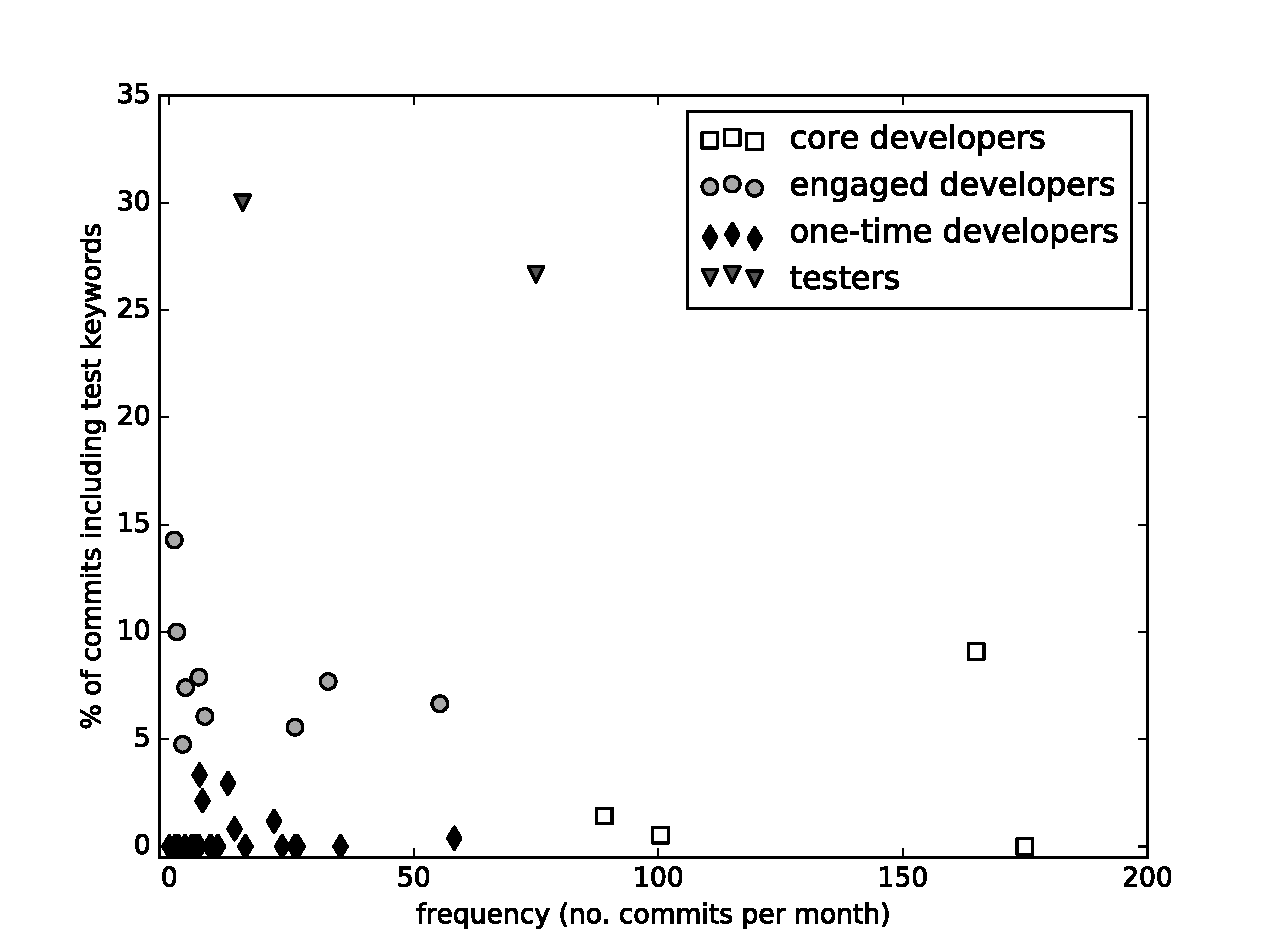
\includegraphics[width=\columnwidth]{ResourceClassification/figures/prom4k_black.pdf}
   \caption{Scatterplot with color-coded clusters, ProM data set}
   \label{fig:prom4k}
\end{figure}

%\todo{shorten to fit into 1 column}

The Camunda data set was analyzed based on the optimal features and classes derived of the Infinica data set. The majority of the users are developers like in the ProM data set. However, it is an open source project and users can commit anything at any time without restrictions. There is a permanently appointed core team which evaluates, selects and integrates commits for the product. The clustering creates similar classes like in the ProM data set and it can be divided into the following four classes as shown in \Cref{fig:camunda4k}.

\begin{itemize}

\item \textbf{Core developers:} The square cluster contains the employed users of the Camunda project. Their commit frequency and absolute number commits is far above the others.

\item \textbf{Engaged developers:} Developers which stay longer with the project are situated in the circle cluster. They are refining their own committed code or they are extending the product in different areas.

\item \textbf{One-time developers:} Similar to the ProM data set the majority of the users belongs to this group and it is represented by the diamond cluster. Code usefull or not is committed typically once and there is no lasting commitment.

\item \textbf{Testers:} Also testers have been identified in the triangle cluster. They already have a lower frequency than developers and therefore it is difficult to make an estimation about their commitment.

\end{itemize}

\begin{figure}
   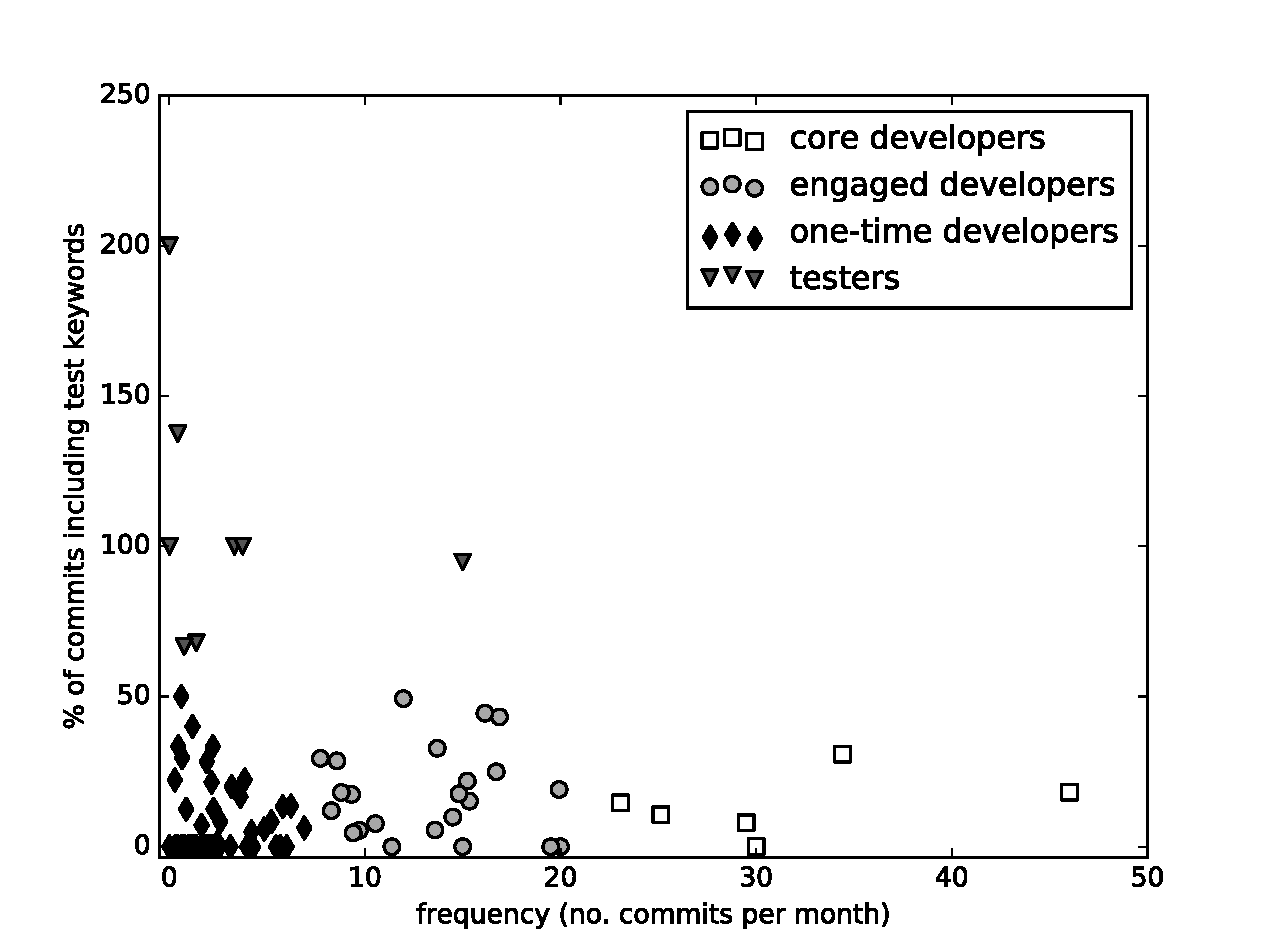
\includegraphics[width=\columnwidth]{ResourceClassification/figures/camunda4k_black.pdf}
   \caption{Scatterplot with colorcoded clusters, Camunda data set}
   \label{fig:camunda4k}
\end{figure}

For the user-based approach no further distinction can be made based on expertise, time in the company, teamwork, development area, project membership, room allocation, etc. In the case of a development from junior to a senior role in the course of the coverage of the log file the respective persons stay within their previous clusters. The associated increase or decrease in commit frequency can not be linked to the development. %since the observations developed in opposite directions.


\begin{figure}
   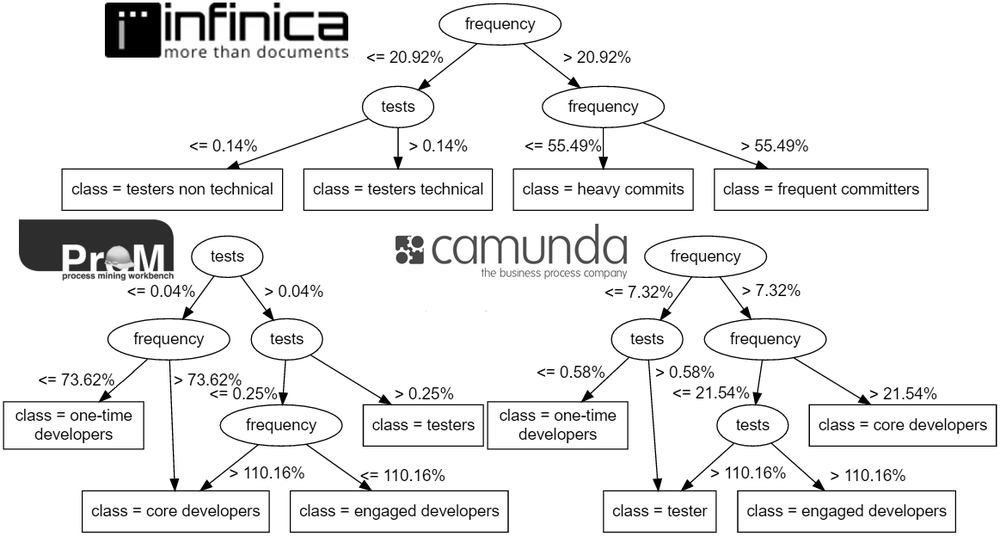
\includegraphics[width=\columnwidth]{ResourceClassification/figures/4ktrees.png}
   \caption{Decision trees, all three data sets}\
   \label{fig:trees}
\end{figure}


Decision trees are an effective tool to display the formation and partitioning of clusters in a tree-like model. The corresponding decision trees for the previous presented k-means clustering shown in \Cref{fig:trees} display the boundaries of the clusters. Due to the differences in the structure of the projects, business vs open source, the data sets share only little similarities.

The Infinica decision tree initially splits the developers and the testers apart based on the commit frequency with a border value of 20.92\%. The developers are split again into subclasses based on the commit frequency, which now separates them at 55.49\% into frequent committers and heavy commits. The testers are split based on test related word occurrences at 0.14\%, where the non technical testers use these words less often than their technical counterparts. On the contrary, the other two trees start separating the subsets right away in different orders without displaying a clean separation between developers and testers from the beginning.

The decision tree model for the commit-based approach is depicted in \Cref{fig:tree}. When comparing its rules with those of our manual classification there are some clear parallels. In the tree the differentiation between web developers and other developers is done with a border value of 36\% for web commits, close to the 40\% threshold of the manual table. Testers are identified having more than 17\% test commits, similar to the 20\% boundary. The decision tree separates the support users from the rest using the vcsManagement type. Looking at the data, this rule is definitely valid for the Infinica data, however as we were not able to provide a definite explanation for this class having higher percentages for that particular type, we can not say if this rule would also apply to other data sets. One possible explanation is that all users have a similar number of vcsManagement commits within a given timeframe, but because the support role has on average a significantly lower number of commits, they account for a higher percentage in the distribution, however this is only an assumption.

\begin{figure}
	\centering
	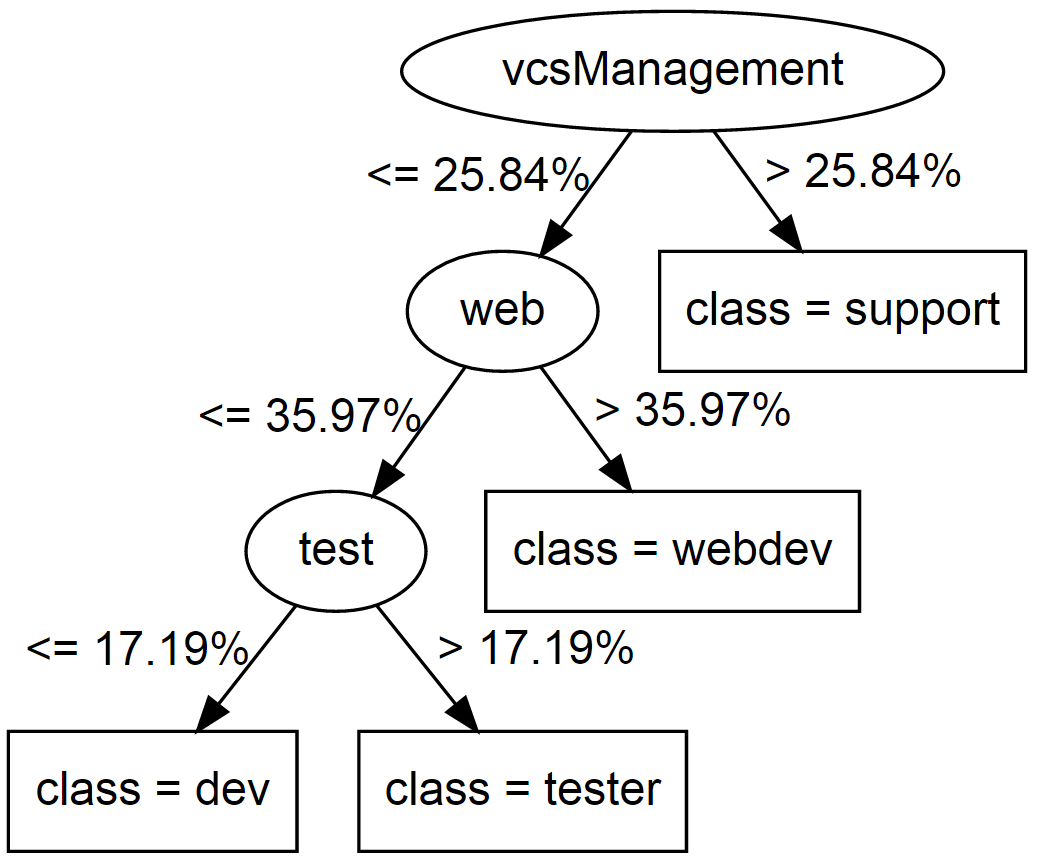
\includegraphics[width=0.6\columnwidth]{ResourceClassification/figures/commit_tree.png}
	\caption{Decision tree, commit based model}
	\label{fig:tree}
\end{figure}

In general the decision tree is more precise, but our manually created rules capture more factors of differentiation and we were able to identify some potential classes which could not be included in the programmatic classification with reasonable effort. A clear advantage of the automated model is that it can be efficiently applied to other data sets. Applying it to the Camunda and ProM data sets provided some verification for our decision tree model. We only included users with five or more commits into the cross validation. For the Prom data set which consisted of 42 users, 35 (83\%) were classified
as developers. This is not surprising as we knew before that the contributors
of open source projects are mostly developers, which was also confirmed by our
contact persons for ProM and Camunda. Six (14\%) were regarded as testers,
which fits to our results in the user-based approach. One remaining user (2\%) was classified as a web developer. As the ProM project has no web component, it makes sense that there are no web developers found by our algorithm. The one we found has only five commits, two of them web commits so this potential misclassification provides no evidence against the quality of the overall approach.

\begin{figure*}[h!t]
	\begin{subfigure}[t]{.5\linewidth}
		\centering
		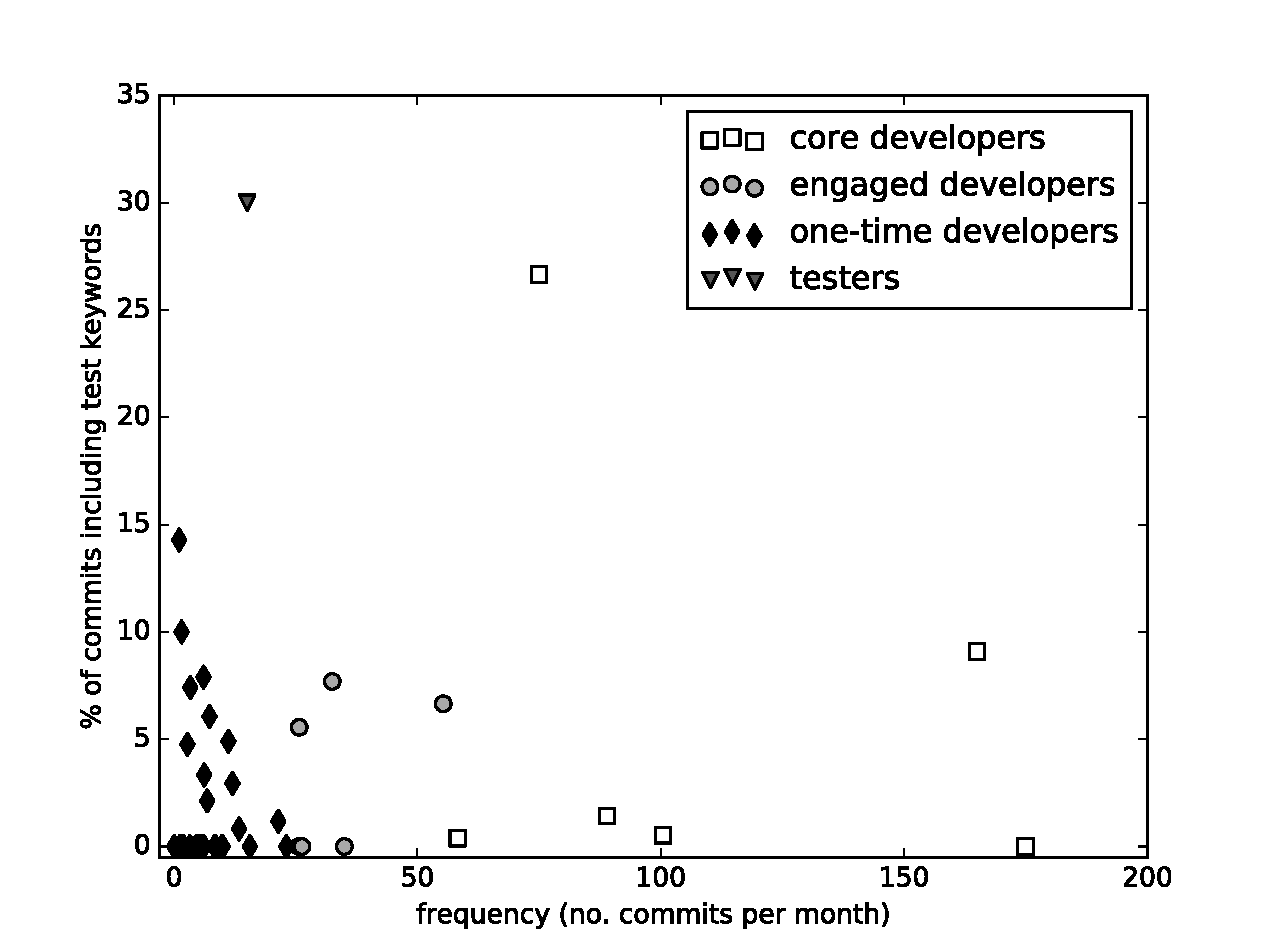
\includegraphics[width=\textwidth]{ResourceClassification/figures/infinica4kpredict_prom_black.pdf}
	\end{subfigure}
	\begin{subfigure}[t]{.5\linewidth}
		\centering
		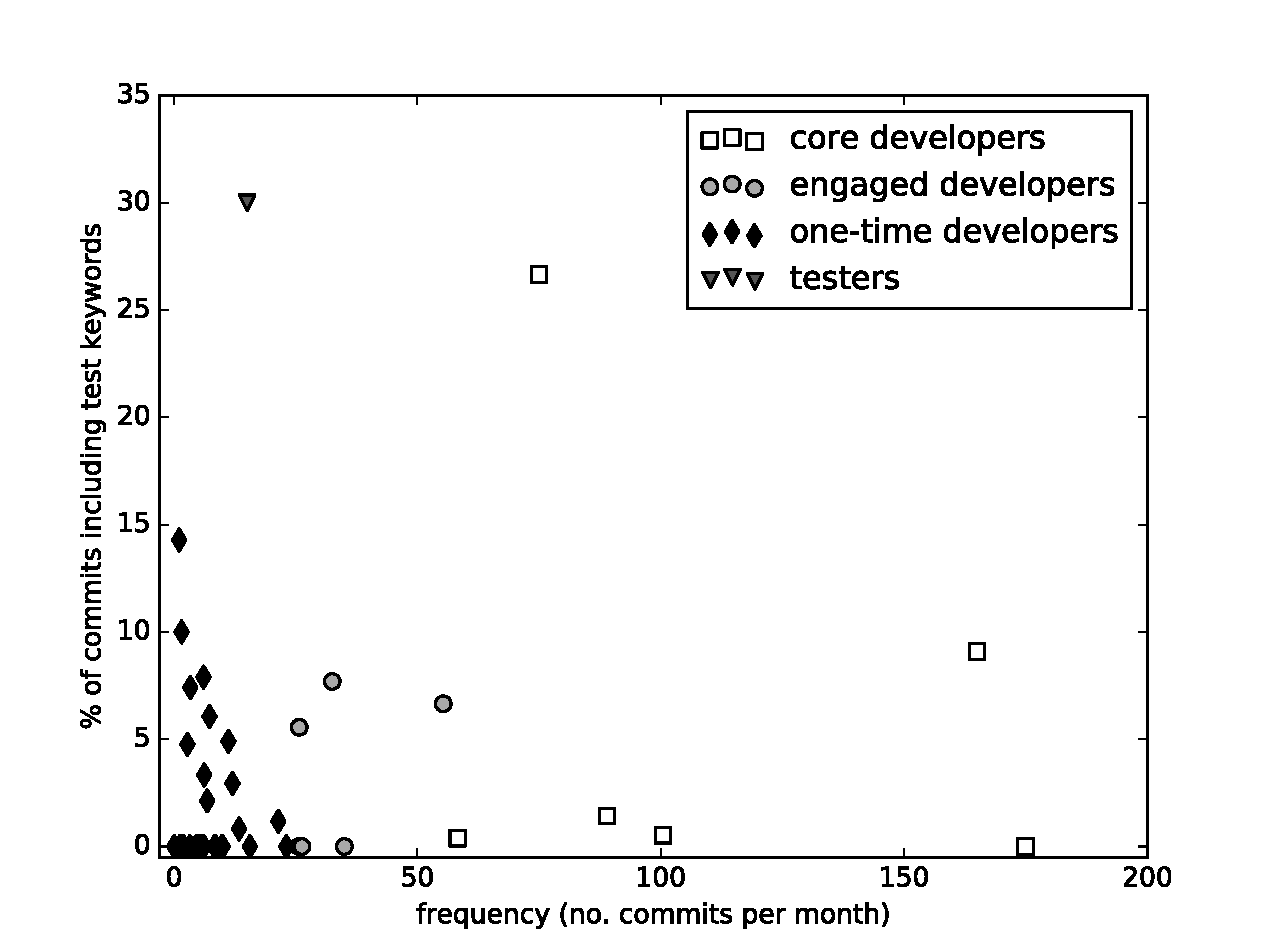
\includegraphics[width=\textwidth]{ResourceClassification/figures/infinica4kpredict_prom_black.pdf}
	\end{subfigure}
	\caption{Classication based on Infinica training set: Prom, Camunda}
	\label{fig:infinica-predict}
\end{figure*}

For the Camunda data the case is similar. Out of 66 total users, 49 (74\%)
percent were regarded as developers, the high number is again explained by the
type of project and was confirmed by the contact person we interviewed. 10 (15\%)
testers were found, also mostly fitting to our knowledge of the data. Contrary
to ProM, there is a web part in the analyzed Camunda project reflected by the
fact that our algorithm found 7 (11\%) web developers. In neither of the two validation data sets a support user was found. This might be due to the differences in the organisational structure between Infinica and the other two or it could stem from the classification rule based on the vcsManagement commit type, which we already discussed as potential source of error. All users in the Camunda and ProM data have below 15 percent vcsManagement commits, too small to fit the support class generated by the decision tree model. However there are other commit types with high percentages, such as build or toolManagement, in Camunda and Prom, which might fit the support class or a similar one.

When validating the model with the Infinica data set and then predicting the ProM and Campunda data set, only moderate results are achieved with the user-based approach as shown in \Cref{fig:infinica-predict}. For the Infinica data set meaningful classes can not be conveyed to the other data sets due to the structural differences of the projects.


For ProM (\Cref{fig:infinica-predict} left) the trained classes are less representative than the ones created when clustering on its own, especially since the ProM data set does not include any designated testers. The prediction of Camunda (\Cref{fig:infinica-predict} right) on the other hand performs better. However, the core developer class now also includes very committed contributors.

Because of the missing designated testers in both test data sets, the initial differentiation between technical and non-technical testers is not possible. Due to the moderate results of user based approach the commit based approach was initiated.


